\documentclass{report}
\usepackage[utf8]{inputenc}


\usepackage[a4paper, total={6in, 8in}]{geometry}


\title{Entwiklung Algorithmus Obere Halswirbelsäule}
\author{Lukas Hörnig}
\date{Oktober 2017}

\usepackage[square,sort,comma,numbers]{natbib}
\usepackage{graphicx}
\usepackage{hyperref}
\usepackage{gensymb}

\begin{document}

\section{Basion Dens Inteval}
\subsection{Definiton}
\begin{figure}
        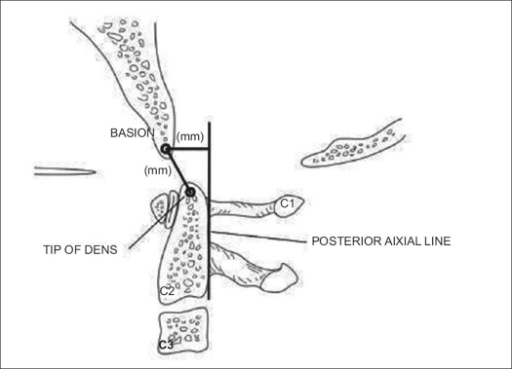
\includegraphics[width=8cm]{BDI.png}
\end{figure}
Definiert als Länge der kürzesten Distanz zwischen dem Mittelpunkt des Basion und der Spitze des Dens in sagitaler Mittelininerekonstruktion in Millimetern.


\subsection{Statistik}
Das BDI zeigt über die Altersgruppen und Geschlechter keine nennenswerte Instabilität \cite{Chaput2011} 
\paragraph{Normalbevölkerung}
\begin{figure}
        \begin{tabular}{l l l l l l l l}
                Studie    & Mean  & SD    & UL 95\% CI & Median   & IQR   & P95 & Cut-Off \\
                Radcliff \cite{Radcliff2010} & 4,59 & 1,68 & 7,88 & 4,56 & 2,11 & 7,52 \\
                Chang \cite{Chang2009} & 6,62 & - & 10.09–12.39 & - & - & - & (93\%) 9,4 \\
                
                
        \end{tabular}
        \end{figure}
\paragraph{Traumapatienten}
\begin{figure}
        \begin{tabular}{l l l l l l l}
                Studie    & Mean  & SD    & UL 95\% CI & Median   & IQR   & P95 \\
                
                        
        \end{tabular}
        \end{figure}
\paragraph{Validität}
\paragraph{Reliabiliät}

\subsection{Patholgischer Wert}
\subsection{Anwendbarkeit}

\section{LMI}
Das LMI zeigt über Altersgruppen und Geschlechter hinweg eine statistisch signifiktante Instabilität \cite{Chaput2011}

\bibliography{../literatur}
\bibliographystyle{dinat}
\end{document}
